    
\begin{frame}[plain]
  \titlepage
\end{frame}


\begin{frame}{Фолдинг и стабильность}

\begin{columns}
\begin{column}{0.7\textwidth}
    \includegraphics[width=1\textwidth]{ddg-scheme.png}
\end{column}
\begin{column}{0.3\textwidth}
Задача дизайна стабильности: указать на замену A>B, которая приведет к положительному $\Delta G_{A>B} $
\end{column}
\end{columns}

\end{frame}

\begin{frame}{Денатурация и агрегация}
\begin{columns}
\begin{column}{0.7\textwidth}
    \includegraphics[height=.85\textheight]{den-aggr.png}
\end{column}
\begin{column}{0.3\textwidth}
    \centering
    35°C<$T_m$≤65°C \\ \vspace{2cm}3 < pH < 10
\end{column}
\end{columns}
\end{frame}

\begin{frame}{Области применения}
    \includegraphics[width=1\textwidth]{ind-application.png}
\begin{columns}
\begin{column}{0.5\textwidth}
Получение коммерчески-применимых ферментов 
\end{column}
\begin{column}{0.5\textwidth}
    Стабилизация терапевтических пептидов и белков
\end{column}
\end{columns}
\end{frame}

\begin{frame}{Направленная эволюция}
    \centering
    \includegraphics[height=.75\textheight]{dir-evolution.png}
\end{frame}

\begin{frame}{Особенности термостабильных белков экстремофилов}
\begin{columns}
\begin{column}{0.4\textwidth}
    В последовательностях:
    \begin{itemize}
        \item Ile, Val, Leu, Trp $\uparrow$
        \item Gly $\downarrow$, Pro $\uparrow$ 
        \item Ser, Gln, Cys, Met $\downarrow$
        \item Больше полярных АК
    \end{itemize}
\end{column}
\begin{column}{0.6\textwidth}
    \includegraphics[width=1\textwidth]{termo.png}\\ \centering \footnotesize{Красные это термофилы}
\end{column}
\end{columns}
\end{frame}


\begin{frame}{Особенности термостабильных белков экстремофилов}
\begin{columns}
\begin{column}{0.3\textwidth}
    В структурах:
    \begin{itemize}
        \item Короткие петли
        \item Меньше полостей
        \item Больше ионных пар на поверхности белка
        \item Плотно упакованные концы
        \item Более протяженные участки вторичной структуры
    \end{itemize}
\end{column}
\begin{column}{0.7\textwidth}
    \includegraphics[width=1\textwidth]{threm-prop.png}
\end{column}
\end{columns}
\end{frame}


\begin{frame}{ProTermDB}
    \includegraphics[height=.8\textheight]{protermdb.png}
\end{frame}

\begin{frame}{Вычислительный дизайн стабильности}
    \centering
    \includegraphics[width=0.49\textwidth]{seq-des.png} 
    \includegraphics[width=0.49\textwidth]{struc-des.png} \\
    \centering
    последовательность \hspace{4cm}  структура
\end{frame}


\begin{frame}{Back-to-consensus}
\begin{columns}
\begin{column}{0.7\textwidth}
    \begin{itemize}
        \item Предполагается, что консенсусные остатки в функционально разнообразных гомологах отвечают за стабильность, а отличия отражают случайные дестабилизирующие мутации, которые оказались нейтральными при отборе
        \item Замена в позиции, отличающейся от гомологов, на консенсусную АК приведет к увеличению стабильности
    \end{itemize}
\end{column}
\begin{column}{0.3\textwidth}
    \includegraphics[width=1\textwidth]{consens.png}
\end{column}
\end{columns}
\end{frame}


\begin{frame}{Востановление предшествиника}
\begin{columns}
\begin{column}{0.6\textwidth}
    \begin{itemize}
        \item Жизнь произошла от термофильных организмов. Предковые гомологи всех белков - термостабильные.
        \item Построение филогенетических деревьев и поиск предковой последовательности приведет к созданию термостабильного белка.
    \end{itemize}
\end{column}
\begin{column}{0.4\textwidth}
    \includegraphics[width=1\textwidth]{ancestral.png}
\end{column}
\end{columns}
\end{frame}


\begin{frame}{Cочетание структурных данных и выравниваний}
\begin{columns}
\begin{column}{0.5\textwidth}
    \begin{itemize}
        \item Рациональный анализ структур
        \item Поиск ковариирующих позиций
        \item Сохранение остатков вторичной структуры
        \item Сохранение функционально важных позиций
    \end{itemize}
\end{column}
\begin{column}{0.5\textwidth}
    \includegraphics[width=1\textwidth]{compl-str-seq.png}
\end{column}
\end{columns}
\end{frame}


\begin{frame}{Оценка ddG единичных замен}
    \centering
    \includegraphics[width=.8\textwidth]{ddg-single.png}
\begin{columns}
\begin{column}{0.3\textwidth}
    \textbf{Physics-based}\\
Оценка межатомных взаимодействий
\end{column}
\begin{column}{0.3\textwidth}
    \textbf{Descriptors-based}\\
    Descriptors-based
Воспроизведение известных структур с применением ML
\end{column}
\begin{column}{0.3\textwidth}
    \textbf{Knowladge-based}\\
Воспроизведение статистических данных
\end{column}
\end{columns}
\end{frame}


\begin{frame}{Оценка ddG единичных замен: CC/PBSA}
\begin{columns}
\begin{column}{0.5\textwidth}
    \begin{itemize}
        \item Physics-based
            \[ \Delta G_{CC/PBSA} =   \Delta G_{EL} + \Delta G_{VdW} + \Delta G_{S}  \]
        \item Вычислительно затратный
    \end{itemize}
\end{column}
\begin{column}{0.5\textwidth}
    \includegraphics[width=1\textwidth]{cc-pbsa.png}
\end{column}
\end{columns}
\end{frame}


\begin{frame}{Оценка ddG единичных замен: PopMusic}
    \begin{columns}
\begin{column}{0.5\textwidth}
    \begin{itemize}
        \item Physics-based
            \[ \Delta \Delta G_{P} = \sum_{i=1}^{13} a_i(A)\Delta\Delta W_i + a_{14}(A)\Delta V_+ + \]
            \[   + a_{15}(A)\Delta V_- + a_{16}(A) \]
        \item WWW available
    \end{itemize}
\end{column}
\begin{column}{0.5\textwidth}
    \includegraphics[width=1\textwidth]{popmusic.png}
\end{column}
\end{columns}
\end{frame}

\begin{frame}{Оценка ddG единичных замен: FoldX}
    \begin{columns}
\begin{column}{0.4\textwidth}
    \begin{itemize}
        \item Physics-based + Knowledge-based
            \[ \Delta G =   \Delta G_{vdw} + \Delta G_{solH} + \Delta G_{solP}  + \]
            \[ + \Delta G_{hbond} + \Delta G_{wb}  + \Delta G_{el} +\]
            \[ + \Delta S_{mc} + \Delta S_{sc}\]
        \item Есть в виде веб-сервера
        \item Умеет работать с ДНК
        \item Умеет работать с димерами
        \item Умеет учитывать стабильность при смене рН или ионной силы раствора
    \end{itemize}
\end{column}
\begin{column}{0.6\textwidth}
    \includegraphics[width=1\textwidth]{foldx.png}
\end{column}
\end{columns}
\end{frame}


\begin{frame}{Оценка ddG единичных замен: Rosetta}
    \begin{columns}
\begin{column}{0.5\textwidth}
    \begin{itemize}
        \item Knowledge-based в сочетании с Монте-Карло динамикой для минимизации структур
        \item До 2016 года для подсчета ddG применялись кастомные протоколы
        \item После - cartesian\_ddG
        \item Вычислительно затратен
    \end{itemize}
\end{column}
\begin{column}{0.5\textwidth}
    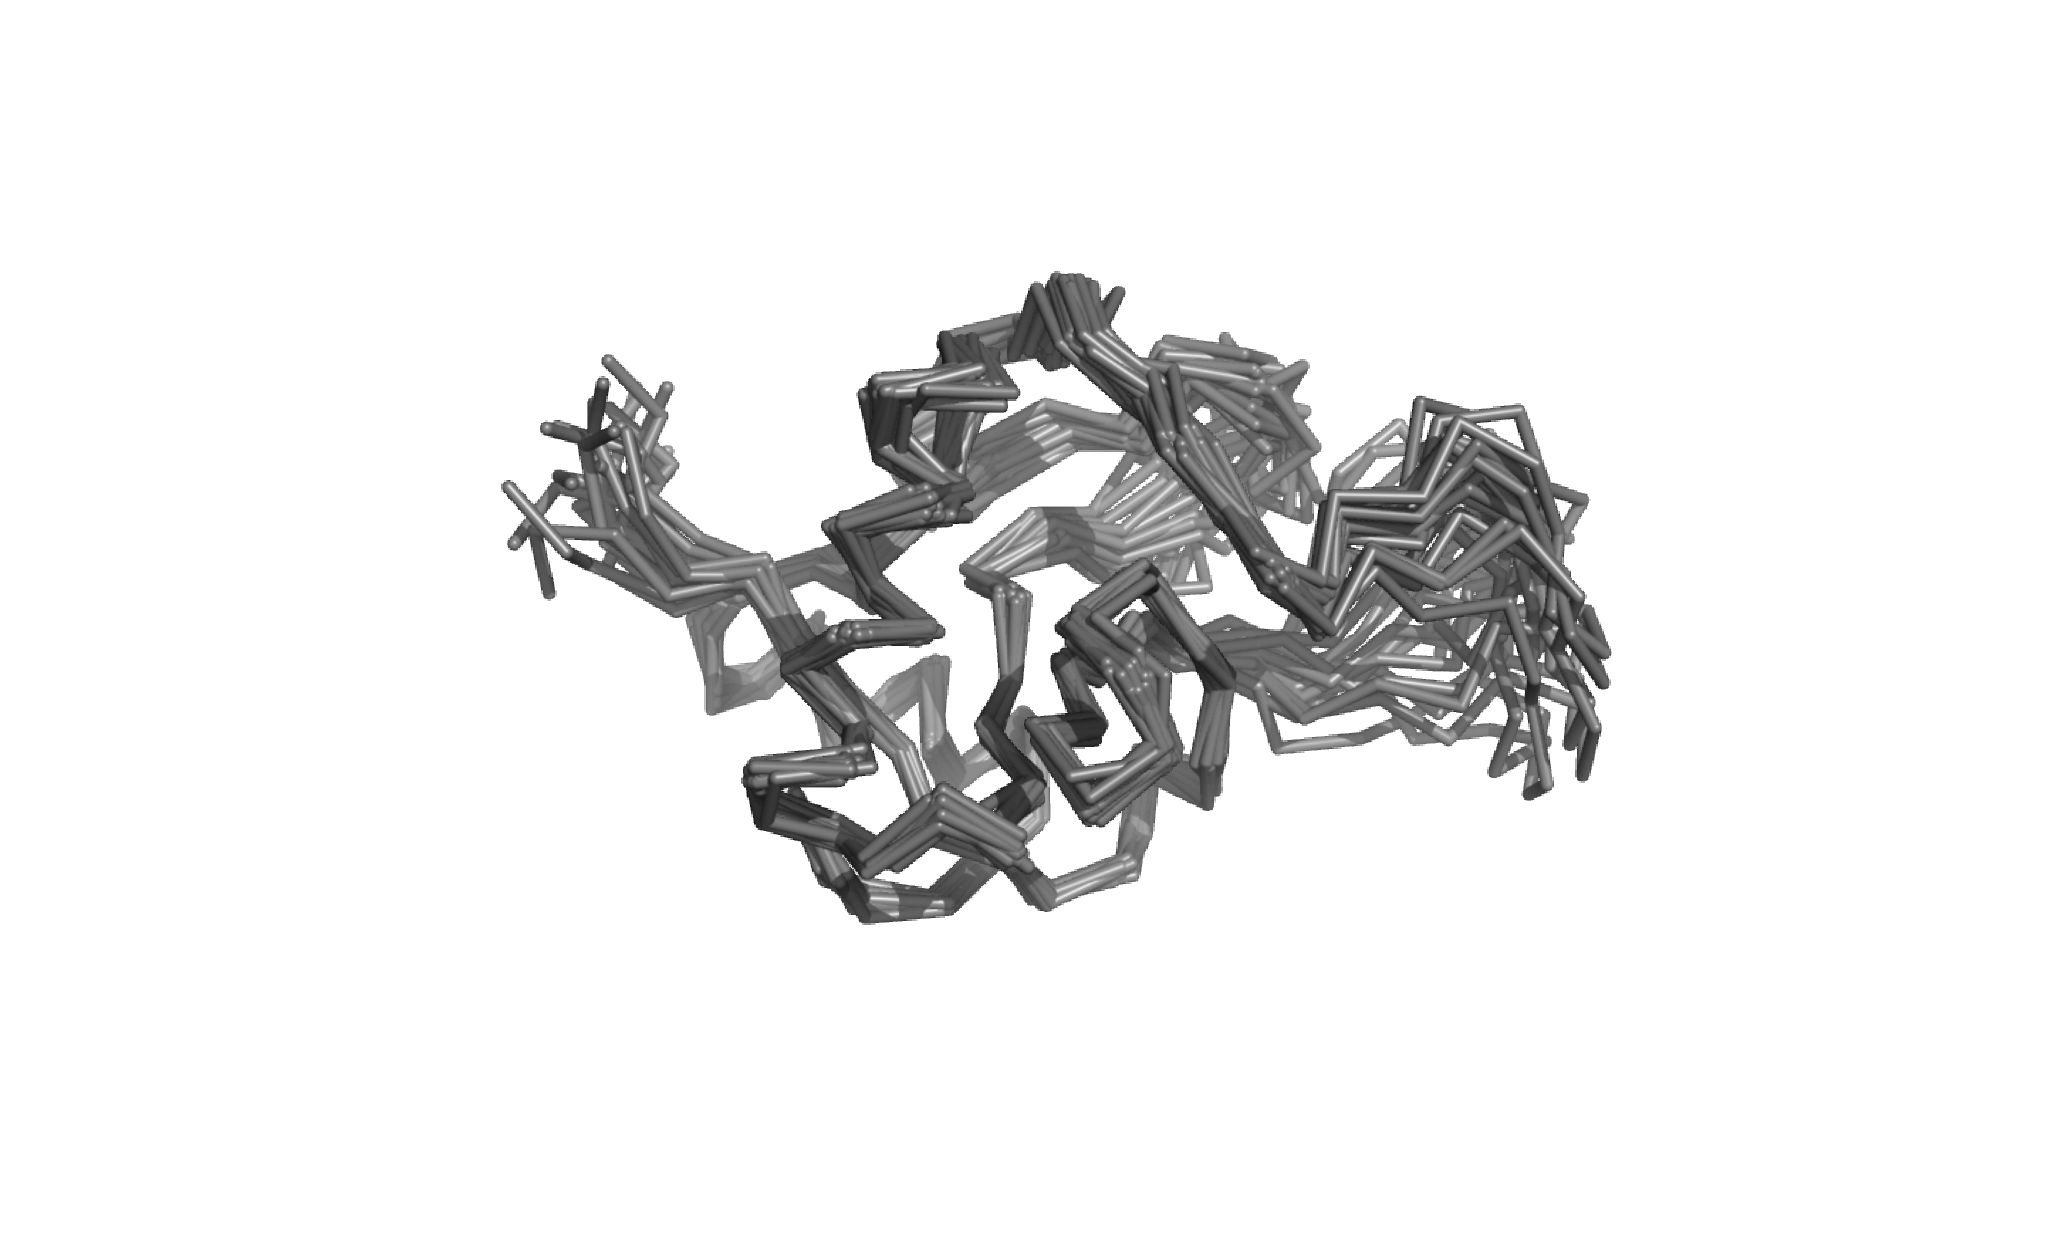
\includegraphics[width=.8\textwidth]{rosetta.png}
\end{column}
\end{columns}
\end{frame}


\begin{frame}{Оценка ddG единичных замен: I-Mutant}
    \begin{columns}
\begin{column}{0.5\textwidth}
    \begin{itemize}
        \item Predictor-based
        \item Support vector machine regression
        \item Есть в виде веб-сервера
        \item Умеет работать с SNP
        \item Умеет работать на последовательности без структуры
    \end{itemize}
\end{column}
\begin{column}{0.5\textwidth}
    \includegraphics[width=1\textwidth]{imutant.png}
\end{column}
\end{columns}
\end{frame}


\begin{frame}{Оценка ddG единичных замен: STRUM}
    \begin{columns}
\begin{column}{0.3\textwidth}
    \begin{itemize}
        \item Predictor-based
        \item Gradient boosting regression
        \item Был в виде веб-сервера - сейчас сервер временно мёртв
    \end{itemize}
\end{column}
\begin{column}{0.7\textwidth}
    \includegraphics[width=1\textwidth]{strum.png}
\end{column}
\end{columns}
\end{frame}

\begin{frame}{Оценка ddG единичных замен: Критика}
    \includegraphics[width=1\textwidth]{critics.png}
\end{frame}

\begin{frame}{Оценка ddG единичных замен: Критика}
    \begin{columns}
\begin{column}{0.5\textwidth}
    \begin{itemize}
        \item Критерий ассиметричности ddG
         $\Delta\Delta G_{WT-> mut} = -\Delta\Delta G_{mut-> WT} $
    \end{itemize}
\end{column}
\begin{column}{0.5\textwidth}
    \includegraphics[width=1\textwidth]{critics-cor.png}
\end{column}
\end{columns}
\end{frame}


\begin{frame}{Дизайн гидрофобных ядер}
    \begin{columns}
\begin{column}{0.5\textwidth}
    \begin{itemize}
        \item Наибольшие успехи - с помощью алгоритмов Rosetta
        \item Получены и стабилизированы неприродные фолды
    \end{itemize}
\end{column}
\begin{column}{0.5\textwidth}
    \includegraphics[width=1\textwidth]{hyp-nucl.png}
\end{column}
\end{columns}
\end{frame}


\begin{frame}{Rosetta VIP}
    \centering
    \includegraphics[width=.7\textwidth]{rosetta-vip.png}\\
10.1073/pnas.1115172109 
\end{frame}

\begin{frame}{Недоупакованное гидрофобное ядро}
    \centering
    \includegraphics[width=.7\textwidth]{hyp-nucl-2.png}\\
    Robust folding of a de novo designed ideal protein even with most of the core mutated to valine.  https://doi.org/10.1073/pnas.2002120117
\end{frame}



\begin{frame}{Внесение заряженных АК}
    \begin{columns}
\begin{column}{0.5\textwidth}
    \begin{itemize}
        \item Формирование солевых мостиков
        \item Негативный дизайн - дестабилизация несвернутых состояний
    \end{itemize}
\end{column}
\begin{column}{0.5\textwidth}
    \includegraphics[height=.8\textheight]{charge.png}
\end{column}
\end{columns}
\end{frame}



\begin{frame}{Дизайн дисульфидных связей}
    \begin{columns}
\begin{column}{0.5\textwidth}
    \begin{itemize}
        \item MODIP, DbD - поиск на основе статистической скоринг-функции
        \item SSbondPre - предиктор на основе нейросети
    \end{itemize}
\end{column}
\begin{column}{0.5\textwidth}
    \includegraphics[height=.8\textheight]{ss-bond.png}
\end{column}
\end{columns}
\end{frame}


\begin{frame}{Дизайн дисульфидных связей с нестандартными АК}
    \begin{columns}
\begin{column}{0.5\textwidth}
    \begin{itemize}
        \item Дисульфидные мостики формируют тиол-содержащие АК
        \item Используются методы биоинформатики для поиска возможных позиций для мутации на тиол-содержащие АК и методы биоинженерии для вставки таких АК в процессе трансляции
    \end{itemize}
\end{column}
\begin{column}{0.5\textwidth}
    \includegraphics[width=1\textwidth]{long-ss.png}
\end{column}
\end{columns}
\end{frame}

\begin{frame}{"network hallucination"}
    \centering
    \includegraphics[width=\textwidth]{halluc}
\end{frame}

\begin{frame}{"network hallucination"}
    \centering
    \includegraphics[width=\textwidth]{halluc-mcmc}
\end{frame}


\begin{frame}{Ограниченные галлюцинации}
    \centering
    \includegraphics[width=0.5\textwidth]{halluc-motif}
    \begin{itemize}
        \item Cложная функцию потери, которая сочетает в себе часть из галлюцинаций с частью реконструкции мотива. 
        \item Подход с ограниченными галлюцинациями требует больших вычислительных ресурсов, поскольку для каждого шага градиентного спуска во время оптимизации последовательности требуется прямой и обратный проход через сеть.
        \end{itemize}
\end{frame}


\begin{frame}{Inpainting}
    \centering
    \includegraphics[width=0.5\textwidth]{inpainting.png}
    \begin{itemize}
        \item Широкий спектр проблем проектирования структуры белков можно аналогичным образом сформулировать как проблемы восстановления недостающей информации 
        \end{itemize}

\end{frame}


\begin{frame}{Inpainting}
    \centering
    \includegraphics[width=0.8\textwidth]{halluc-inp.png}

\end{frame}

\begin{frame}{RFjoint}
    \centering
    \includegraphics[width=\textwidth]{rfjoint.png}

\end{frame}

\begin{frame}{Inpainting}
    \centering
    \includegraphics[width=\textwidth]{rfjoint-thermo.png}

\end{frame}

\begin{frame}{Rapid protein stability prediction}
    \centering
    \includegraphics[width=0.9\textwidth]{rasp-scheme.png}
\end{frame}
\begin{frame}{Заключение}
    \begin{itemize}
        \item  В процессе дизайна стабильности белка приходится иметь дело со сложным процессом фолдинга белка, предсказать который пока невозможно - приходится аппроксимировать
        \item Выборки для обучения методов предсказания ограничены
        \item  Несмотря на локальные успехи - мало системных универсальных методов
    \end{itemize}
\end{frame}

